\section{S5 -- Charakterystyka wybranej techniki wirtualizacji}

\textbf{Wirtualizacja} jest to metodologia polegająca na dzieleniu zasobów komputera na wiele środowisk. Działają one poprzez zastosowanie jednej lub wielu technologii, np. sprzętowe lub softwarowe partycjonowanie, tworzenie maszyny wirtualnej, przydzielanie czasu.

\begin{figure}[H]
	\centering
	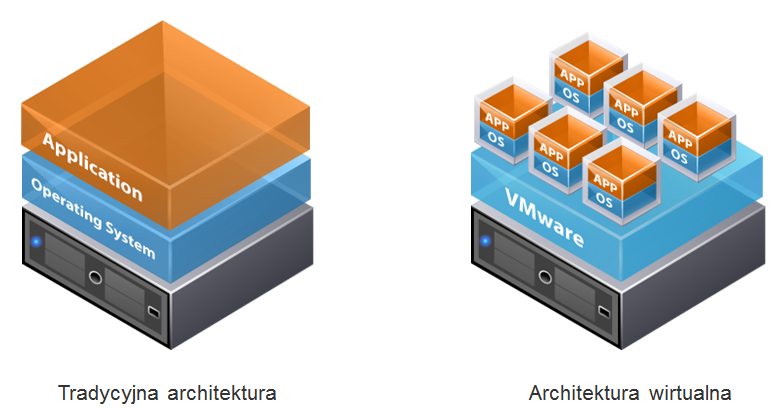
\includegraphics[scale=0.45]{s5_wirtualizacja.png}
	\caption{Wirtualizacja serwerów}
\end{figure}


\begin{itemize}
	\setlength\itemsep{1pt}
	\item \textbf{Obszary wirtualizacji:}
	\item \textbf{Wirtualizacja serwerów} (ang. \textit{Server Virtualization}) – technologia ta  umożliwia wielu aplikacjom działanie na wielu systemach operacyjnych uruchomionych na tym samym fizycznym serwerze z wykorzystaniem wolnej mocy. Dzięki temu można w pełni wykorzystać moc obliczeniową i zasobową serwerów, stawiając kolejne maszyny wirtualne na jednym fizycznym serwerze – zamiast kupować kolejne serwery fizyczne. Dodatkową zaletą jest też szybsze dostarczenie usług dla biznesu w ciągu bardzo krótkiego czasu tworzenia nowego wirtualnego systemu operacyjnego gotowego do pracy. Ponadto podstawowe zadania konserwacyjne związane z serwerami są znacznie uproszczone i przyśpieszone.
	\item \textbf{Wirtualizacja stacji roboczych} (utrzymywana na kliencie) (ang. \textit{Client-HostedDesktop Virtualization}) – to rodzaj wirtualizacji, która oddziela system operacyjny kliencki od sprzętu fizycznego i umożliwia uruchomienia maszyn wirtualnych na jednym komputerze PC obok klienckiego systemu operacyjnego hosta. Może być centralnie zarządzana, a obrazy maszyn wirtualnych mogą być dostarczane również centralnie. Technologię tę stosuje się wtedy, gdy zachodzi potrzeba zapewnienia zgodności aplikacji z systemem operacyjnym. Aplikacje są zainstalowane w maszynie wirtualnej i tam wykonuje się ich kod. Dostarczenie aplikacji do użytkownika odbywa się najczęściej w trybie seamless, czyli bez dodatkowej otoczki pulpitu – jedynie widok samej aplikacji.
	\item \textbf{Wirtualizacja stacji roboczych} (utrzymywana na serwerze)(ang. \textit{Server-Based Desktop Virtualization}) – znana bardziej pod nazwą \textbf{Wirtualna infrastruktura stacji roboczych} (ang. \textit{Virtual Desktop Infrastructure – VDI}). Jest to przeniesienie klasycznego środowiska pracy użytkownika, opartego na stacjach roboczych, do centrum przetwarzania danych, gdzie stacja robocza jest uruchomiona w postaci maszyny wirtualnej, a dostęp do niej zapewniony jest drogą sieciową. Połączenie może być zrealizowane z dowolnego komputera PC, laptopa lub cienkiego klienta, który jest preferowaną formą dostępu do VDI. Sam w sobie VDI nie jest jedną technologią – to połączenie kilku niezależnych rozwiązań, które w podstawowej architekturze łączy ze sobą wirtualizację serwerów z wirtualizacją prezentacji.
	\item \textbf{Wirtualizacja sieci} (ang. \textit{Network Virtualization}), którą można podzielić na dwa rodzaje – zewnętrzną oraz wewnętrzną. Zewnętrzna wirtualizacja sieci to znana od lat technologia VLAN (802.1Q), czyli logiczny podział segmentów sieci na fizycznym sprzęcie sieciowym przez znakowanie ramek. Wewnętrzna natomiast to rozwiązanie polegające na tworzeniu wirtualnych przełączników i portów na poziomie hiperwizora. Takie zwirtualizowane przełączniki dostarczają komunikację sieciową dla maszyn wirtualnych oraz łączą je z zewnętrzną fizyczną siecią.
	\item \textbf{Chmura prywatna} (ang. \textit{Private Cloud}) to realizacja koncepcji chmury wewnątrz własnej firmy, czyli na własnych serwerach i własnym oprogramowaniu. W wersji podstawowej w chmurze prywatnej można zrealizować model infrastruktury jako usługi (ang. Infrastructure as a Service  – IaaS). Bardziej złożone chmury prywatne mogą realizować model platformy jako usługi (ang. Platform as a Service – PaaS). Odbiorca mocy obliczeniowej lub zasobów nie wie tak naprawdę, w którym miejscu infrastruktury firmy się znajduje, gdyż jego przestrzeń może dynamicznie wędrować między serwerami oraz dynamicznie się skalować. Podsumowując, chmura prywatna to nic innego, jak usługi przetwarzania w chmurze świadczone przez dział IT dla własnej firmy.
\end{itemize}

\begin{itemize}
	\setlength\itemsep{1pt}
	\item[] \textbf{Zalety Wirtualizacji: }
	\item redukcja kosztów w aspekcie długoterminowym,
	\item ograniczenie rozrostu serwerowni,
	\item konsolidacja zasobów,
	\item elastyczność przydziału zasobów,
	\item łatwe testowanie nowych aplikacji oraz sieci komputerowych,
	\item możliwość uruchomienia większej ilości usług na jednym sprzęcie.
	\item korzystanie ze starszych aplikacji, niekompatybilnych z obecnie produkowanym sprzętem czy nowymi systemami,
	\item dostępność na bardzo wysokim poziomie.
\end{itemize}
	
\begin{itemize}
	\setlength\itemsep{1pt}
	\item[] \textbf{Wady: }
	\item Infrastruktura informatyczna, musi być bardzo wydajna i niezawodna,
	\item koszt inwestycji w mocne serwery,
	\item zakup licencji,
	\item wirtualne maszyny mogą być w niektórych przypadkach mniej wydajne od tradycyjnych rozwiązań,
	\item potrzeba wykwalifikowanej kadry zarządzającej.
\end{itemize}
	
My podczas zajęć korzystaliźmy z wirtualizacji VirtualBoxa, emulując np. Windowsa 7, czy CentOS-a.

\begin{itemize}
	\setlength\itemsep{1pt}
	\item[] \textbf{Typy wirtualizacji}
	\item \textbf{Parawirtualizacja} – technika wirtualizacji, w której wirtualizowany system operacyjny (Gość – ang. \textit{Guest}, Partycja – ang. \textit{Partition} lub Domena – ang. \textit{Domain}) współpracuje ze środowiskiem operacyjnym komputera w zakresie obsługi tych elementów sprzętowych, których obsługa kolidowałaby z działalnością innych środowisk wirtualizowanych.
	
	\textbf{Parawirtualizacja} jest to jedna lub wiele maszyn wirtualnych działających obok systemu host. Parawirtualizacja korzysta z hypervisora typu 1, monitor działa tutaj bezpośrednio na sprzęcie i udostępnia go (lub nie) systemom guest. Jeden z wirtualizowanych systemów pełni rolę zarządzającą, może rozdzielać zasoby pośród pozostałych systemów i pełnić pełną kontrolę nad maszyną wirtualną i jej zasobami. System, który mógłby być uruchomiony jako guest za pomocą parawirtualizacji, musi mieć zmodyfikowane jądro w taki sposób, aby zamiast odwołań do sprzętu, jak również standardowych odwołań do sprzętu, które są niedozwolone podczas parawirtualizacji, trzeba używać odwołań typu hypercall. Odwołanie to po prostu interfejs pomiędzy monitorem a systemami guest. Mechanizm zapewnia tutaj bardzo dobrą wydajność, bardzo zbliżoną do natywnego działania systemu. Bardzo dobra wydajność systemów guest oraz łatwość w modyfikowaniu jądra systemu guest w celu przystosowania go do parawirtualizacji jest jego zaletą. Natomiast wadą jest konieczność modyfikowania systemu guest, ponieważ nie zawsze jest możliwe uzyskanie takiej wydajności. Niestety modyfikacja jądra niesie za sobą również koszty związane z dostosowaniem systemu guest do odpowiedniego hypervisora oraz musimy tę procedurę ponowić dla każdego innego hypervisora. Implementacją parawirtualizacji w postaci VMI (Virtual Machine Interface) jest interfejs komunikacji pomiędzy systemem guest a hypervisorem proponowanym przez VMware. Można również powiedzieć, że VMI jest to próba ujednolicenia interfejsu dla wirtualizacji. Celem było także stworzenie jednego interfejsu komunikacji, który byłby zaimplementowany na wielu hypervisorach i w miarę łatwa byłaby implementacja na systemach guest. Zaletą VMI jest to, że implementacja ta nie jest przynależna do jednego hypervisora tylko jest otwarta. Implementacja systemu guest dałaby raz możliwość uruchomienia go we wszystkich liczących się hypervisorach.
	
	\item \textbf{Pełna wirtualizacja} – technika wirtualizacji, w której wirtualizowany system operacyjny (gość) ma wrażenie, że działa na prawdziwym, fizycznym sprzęcie (komputerze). W rzeczywistości odwołania wirtualizowanego systemu operacyjnego (gościa) do tych elementów fizycznych komputera, które kolidowałyby z działalnością innych środowisk wirtualizowanych lub systemu operacyjnego gospodarza (ang. host), są przechwytywane przez oprogramowanie wirtualizacyjne, a następnie emulowane. Emulacja taka spowalnia pracę wirtualizowanego środowiska, dlatego pożądane jest sprzętowe wspomaganie wirtualizacji.
	
	\textbf{Pełna wirtualizacja} pozwala nam na wirtualizowanie dowolnie wybranego niezmodyfikowanego systemu operacyjnego. Największą zaletą pełnej wirtualizacji jest to, iż nie narzuca ona nam żadnych ograniczeń ani wymagań co do systemu guest. Wydajność w takim rozwiązaniu jest niestety mniejsza niż w przypadku parawirtualizacji. Zarówno za pomocą hypervisora typu 1, jak i typu 2 może być zrealizowana pełna wirtualizacja. Głównym wyzwaniem pełnej wirtualizacji jest realizowanie i przechwytywanie uprzywilejowanych instrukcji jądra guest, tak jak na przykład operacja I/O, przerwań czy operacji na pamięci. Większość instrukcji systemu guest wykonywana jest bezpośrednio na procesorze przez hypervisora, natomiast te instrukcje, które wychodzą poza uprawnienia systemu guest, jak też odwołują się do sprzętu, powinny być przechwycone i emulowane. W przypadku kiedy zostanie użyty hypervisor typu 1 wymagane jest odpowiednie rozszerzenie sprzętowe, które umożliwia wirtualizację. Pełną wirtualizację określa się również pojęciem natywna wirtualizacja oraz wirtualizacja wspierana sprzętowo. Jeśli do pełnej wirtualizacji użyjemy hypervisora typu 2, to będziemy ją realizować przez mechanizmy takie jak binary translation oraz direct execution, często ze wsparciem pamięci podręcznej tych transakcji w postaci cache, można również użyć kompilacji instrukcji just in time.
\end{itemize}

